\documentclass{beamer}
\usepackage{listings}
\usepackage{booktabs}
\usepackage{tikz} 
\usepackage{chronology}
\usetikzlibrary{decorations.pathreplacing,calligraphy}
\usetikzlibrary{positioning, arrows.meta, calc}

\usepackage{array}
\usepackage{appendixnumberbeamer}

\usepackage{subcaption}
\usepackage[font=small,labelfont=bf,
   justification=justified,
   format=plain]{caption}

\usetikzlibrary{positioning}

\usepackage{lipsum} 
\setbeamersize{text margin left=5mm,text margin right=5mm} 
\setbeamertemplate{caption}{\raggedright\insertcaption\par}
\setbeamertemplate{footline}[frame number]
\graphicspath{{../../../../../Dropbox/Lawsuits Asymmetry/output}}
% \usepackage{beamerthemesplit} // Activate for custom appearance

\title{Costs of Time}
\author{Tyler Jacobson}
\date{\today}
\AtBeginSection[]{
  \begin{frame}[noframenumbering]
  \vfill
  \centering
  \begin{beamercolorbox}[sep=8pt,center,shadow=true,rounded=true]{title}
    \usebeamerfont{title}\insertsectionhead\par%
  \end{beamercolorbox}
  \vfill
  \end{frame}
}
\beamertemplatenavigationsymbolsempty

\begin{document}
\maketitle

\begin{frame}
    \frametitle{Agenda}
   \begin{itemize}
    \item Stylized Model
    \item Entitlement Pipeline: Facts + Lessons
    \item Entitlements: Avoiding political uncertainty
   \end{itemize} 
   Did see suggestive evidence in NYC that experience reduces permit withdrawal rates (6\% for first project 2\% for tenth project)
\end{frame}

\section{Entitlement Intuition}

\begin{frame}
    \frametitle{Risk of Failure}
   \begin{itemize}
    \item Proposing a development project involves building a coalition of size $Q$: scales with size.
    \item Each member of the coalition succeeds at its task with probability:
    $$\delta^T$$
    \item More time between when the coalition forms and when building can occur leads to higher risk of failure. 
    \item Likelihood of Success is:
    $$\prod_{q=1}^Q \delta^T = \delta^{QT}$$ 
   \end{itemize} 
\end{frame}

\begin{frame}
    \frametitle{Developer's Proposal Decision}
    \begin{itemize}
        \item Project of size $Q$ with profits $\pi(Q)$ has expected return:
   $$\beta^T  \delta^{QT} \pi(Q)$$
   \item Risk of failure adjusts discount factor from:
    $$\beta \to \beta\delta^Q$$
   \item The first order condition with respect to $Q$ is:
   $$\beta^T \delta^{QT}T\ln(\delta) \pi(Q) + \beta^T  \delta^{QT} \pi'(Q)=0 $$
   $$T\ln(\delta)\pi(Q) + \pi'(Q) = 0$$
   \item Long approval timeline shifts projects off ideal FOC: $\pi'(Q)=0$
    \end{itemize}
\end{frame}


\section{Entitlement Pipeline: Facts}

\begin{frame}
    \frametitle{Entitlements Rarely Outright Denied}
\begin{figure}[H]
   \centering
   \includegraphics[width=0.9\textwidth]{sum_stats/bar_determination_outcomes.pdf}
  \end{figure}
\end{frame}

\begin{frame}
    \frametitle{Not All Entitlements Equal: Ten Most Common}
\begingroup
\renewenvironment{table}[1][]{}{}
\renewcommand{\caption}[2][]{}
\centering\resizebox{.9\linewidth}{!}{\input{../../../../../Dropbox/Lawsuits Asymmetry/output/sum_stats/entitlement_top10_common}}
\endgroup
\end{frame}

\begin{frame}
    \frametitle{Not All Entitlements Equal: Ten Longest}
\begingroup
\renewenvironment{table}[1][]{}{}
\renewcommand{\caption}[2][]{}
\centering\resizebox{.9\linewidth}{!}{\input{../../../../../Dropbox/Lawsuits Asymmetry/output/sum_stats/entitlement_top10_longest}}
\endgroup
\end{frame}

\begin{frame}
    \frametitle{Longer Cases Have More Withdrawals}
\begin{figure}[H]
   \centering
   \includegraphics[width=0.9\textwidth]{sum_stats/scatter_cases_withdraw_length.pdf}
  \end{figure}
\end{frame}


\begin{frame}
    \frametitle{Share of Units in ``Complicated'' Entitlements Falling}
\begin{figure}[H]
   \centering
   \includegraphics[width=0.9\textwidth]{sum_stats/units_complicated_entitlements_ts.pdf}
  \end{figure}
\end{frame}


\begin{frame}
    \frametitle{Share of Entitlements Built Over Time}
    \begin{figure}[H]
        \includegraphics[width=.9\textwidth]{sum_stats/ts_matched_ym.pdf}
    \end{figure}
\end{frame}

\begin{frame}
    \frametitle{Longer Approved Projects More Likely to Be Unbuilt }
    \begin{figure}[H]
        \includegraphics[width=.9\textwidth]{sum_stats/binscatter_match_length.pdf}
    \end{figure}
\end{frame}

\begin{frame}
    \frametitle{Regression Estimates}
\begingroup
\renewenvironment{table}[1][]{}{}
\renewcommand{\caption}[2][]{}
\centering\resizebox{.9\linewidth}{!}{\input{../../../../../Dropbox/Lawsuits Asymmetry/output/sum_stats/tab_matched_regressions.tex}}
\endgroup
\end{frame}

\begin{frame}
    \frametitle{Nominal Rent Growth Positive}
    \begin{figure}[H]
        \includegraphics[width=.9\textwidth]{sum_stats/hist_rent_growth.pdf}
    \end{figure}
\end{frame}


\begin{frame}
    \frametitle{Lessons}
    \begin{itemize}
    \item Large and long approval projects less likely to be completed: hard to distinguish whether it's something about the approval process vs something inherent to the project
    \begin{itemize}
        \item Ideal: instrument for time in approval process using congestion---likely to be underpowered
    \end{itemize}
    \item Rent growth a negative predictor of entitlement completion. Two stories
    \begin{itemize}
        \item Reverse causality: completed entitlements are a shift in supply and lower rents
        \item High upfront costs: little speculative behavior $\implies$ potentially missing projects
    \end{itemize} 
    \item While rents are weak predictors of building, time series suggests cost increases are very important
    \item Next Steps: hazard model, continue work on predicting profits at proposal, use that to see if observably speculative behavior (projects unlikely to pencil today but would in the future), write.
    \end{itemize}
\end{frame}


\section{Mechanism: Political Risk}

\begin{frame}
    \frametitle{Lessons}
    \begin{itemize}
    \item Story: many stakeholders and long timelines create risk of one stakeholder failing
    \item Observable mechanism: council member or mayor championing the project may leave office
    \item LA has member deference like in Chicago, NYC but only 15 Council Districts
    \item Some suggestive evidence that developers propose complicated projects with confidence over decisionmaker
    \end{itemize}
\end{frame}

\begin{frame}
    \frametitle{Council Members in District 4}
    \begin{figure}[H]
        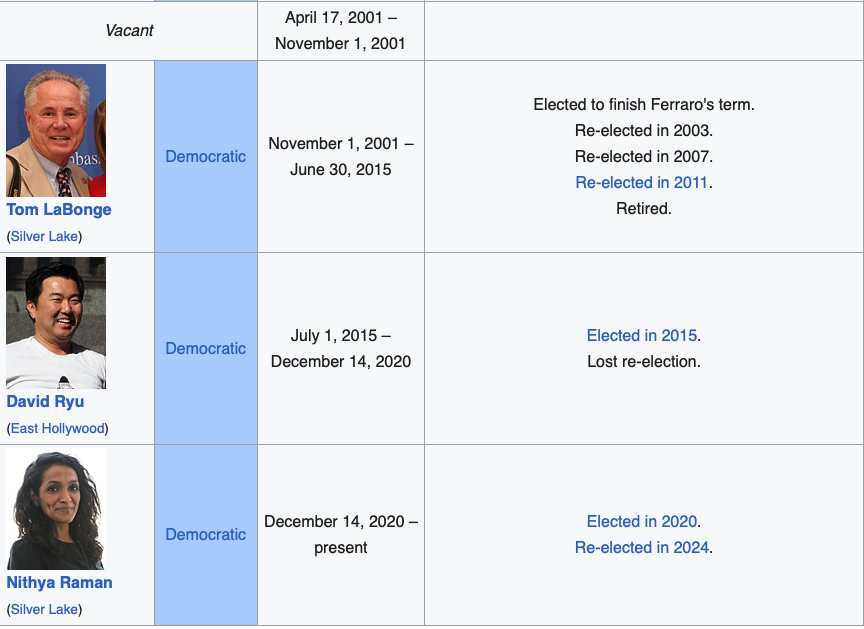
\includegraphics[width=.9\textwidth]{wikipedia_district4.png}
    \end{figure}
\end{frame}


\begin{frame}
    \frametitle{Rising Chance of New Council Member Near End of Tenure}
    \begin{figure}[H]
        \includegraphics[width=.9\textwidth]{politicians/empirical_politician_change_time_remaining.pdf}
    \end{figure}
\end{frame}

\begin{frame}
    \frametitle{Major Entitlements Proposed Bimodally}
    \begin{figure}[H]
        \includegraphics[width=.9\textwidth]{politicians/kdensity_time_remaining.pdf}
    \end{figure}
\end{frame}


\begin{frame}
    \frametitle{Major Entitlements At District Level}
    \begin{figure}[H]
        \includegraphics[width=.9\textwidth]{politicians/complicated_filed_by_cd.pdf}
    \end{figure}
\end{frame}


\begin{frame}
    \frametitle{Major Entitlements At District Level: CD FEs}
    \begin{figure}[H]
        \includegraphics[width=.9\textwidth]{politicians/complicated_filed_by_cd_fes.pdf}
    \end{figure}
\end{frame}


\begin{frame}
    \frametitle{Major Entitlements At District Level: CD+Monthly FEs}
    \begin{figure}[H]
        \includegraphics[width=.9\textwidth]{politicians/complicated_filed_by_cd_ym_fes.pdf}
    \end{figure}
\end{frame}

\begin{frame}
    \frametitle{Half as Many Major Projects at End of Tenure}
    \begin{figure}[H]
        \includegraphics[width=.9\textwidth]{politicians/complicated_filed_by_cd_ym_fes.pdf}
    \end{figure}
\end{frame}

\begin{frame}
    \frametitle{Sample Issues}
    \begin{itemize}
        \item Analysis in LA limited by 15 districts and four year terms
        \item Parcel analysis could be more precise
        \item Could supplement with additional data:
        \begin{enumerate}
            \item Land Use Changes in NYC: have data in hand
            \item Chicago Planned-Developments/Zoning Map Changes: connection at planning department but not sure if worth reaching out.
        \end{enumerate}
    \end{itemize}
\end{frame}
\section{NYC Learning by Doing}
\begin{frame}
    \frametitle{Sample Issues}
    \begin{itemize}
        \item Analysis in LA limited by 15 districts and four year terms
        \item Parcel analysis could be more precise: complementary to above entitlements analysis
        \item Could supplement with additional data:
        \begin{enumerate}
            \item Land Use Changes in NYC: have data in hand
            \item Chicago Planned-Developments/Zoning Map Changes: connection at planning department but not sure if worth reaching out.
        \end{enumerate}
    \end{itemize}
\end{frame}

\end{document}